% Titre : fonctions
% Filiere : BCPST
% Difficulte : 
% Type : TD 
% Categories :fonctions
% Subcategories : 
% Keywords : fonctions




\begin{exercice}  \;
\textbf{(Valeurs absolues)}
On consid\`ere les fonctions $f$ et $g$ d\'efinies sur $\R$ par
$$f:\ x\mapsto |2x-3|+|x-5|\quad \hbox{et}\quad g:\ x\mapsto |2x^2-5|-|x^2-1|.$$
Simplifier les expressions de $f(x)$ et de $g(x)$ en fonction des valeurs de $x$. En d\'eduire les repr\'esentations graphiques de ces deux fonctions.
\end{exercice}


\%\%\%\%\%\%\%\%\%\%\%\%\%\%\%\%\%\%\%\%
\%\%\%\%\%\%\%\%\%\%\%\%\%\%\%\%\%\%\%\%
\%\%\%\%\%\%\%\%\%\%\%\%\%\%\%\%\%\%\%\%



\begin{correction}  \;
\begin{enumerate}
\item \'Etude de $f$: on fait un tableau donnant les valeurs de $f$ selon la valeur de $x$: 
\begin{center}
 \begin{tikzpicture}
 \tkzTabInit{ $x$          /1,%
      $| 2x-3|$   /1,
      $| x-5 | $  /1,
       $f(x)$       /2}%
     { $-\infty$,$\ddp\frac{3}{2}$,$5$,$+\infty$}%
   \tkzTabLine{ ,-2x+3,0,2x-3,t,2x-3,}         
   \tkzTabLine{ ,-x+5,t,-x+5,0,x-5,}       
   \tkzTabLine{ ,-3x+8,t,x+2,t,3x-8,}                 
\end{tikzpicture}
\end{center}
On peut alors tracer la fonction qui correspond \`{a} 3 bouts de droite, qui se rejoignent en $\ddp\frac{3}{2}$ et en $5$.
\item \'Etude de $g$: On fait de m\^{e}me pour la fonction $g$:
\begin{center}
 \begin{tikzpicture}[scale=0.9]
 \tkzTabInit{ $x$          /1.2,%
      $|2x^2-5|$   /1.2,
      $| x^2-1| $  /1.2,
       $f(x)$       /2}%
     { $-\infty$ ,$-\ddp\sqrt{\ddp\frac{5}{2}}$,$-1$,$1$,$\ddp\sqrt{\ddp\frac{5}{2}}$,$+\infty$}%
   \tkzTabLine{ ,2x^2-5,0,5-2x^2,t,5-2x^2,t,5-2x^2,0,2x^2-5}         
   \tkzTabLine{ ,x^2-1,t,x^2-1,0,1-x^2,0,x^2-1,t,x^2-1,}       
   \tkzTabLine{ ,x^2-4,t,-3x^2+6,t,-x^2+4,t,-3x^2+6,t,x^2-4,}                 
\end{tikzpicture}
\end{center}






%On peut alors tracer la fonction.
\end{enumerate}
%\begin{center}
%\begin{minipage}[c]{0.4\textwidth}
%\begin{center}
%\includegraphics[width=0.8\linewidth]{./ex12_1.eps} 
%\end{center}
%\end{minipage}
%\begin{minipage}[c]{0.4\textwidth}
%\begin{center}
%\includegraphics[width=0.8\linewidth]{./ex12_2.eps} 
%\end{center}
%\end{minipage}
%\end{center}
\end{correction}
%--------------------------------------------------
%------------------------------------------------
